\documentclass[12pt]{article}

% --- Pacotes ---
\usepackage[utf8]{inputenc}
\usepackage[english]{babel}
\usepackage{graphicx}
\usepackage{float}
\usepackage{amsmath}
\usepackage{amssymb}
\usepackage{bm}
\usepackage{xcolor}
\usepackage{booktabs}
\usepackage{mathtools}
\usepackage{url}

% --- Macros for the Chapman-Enskog derivation (lbm_teoria.tex) ---
\newcommand{\dt}{\Delta t}
\newcommand{\cs}{c_s}
\newcommand{\uph}{\bm{u}}
\newcommand{\Ftot}{\bm{F}_{\mathrm{tot}}}
\newcommand{\Fext}{\bm{F}_{\mathrm{ext}}}
\newcommand{\Fcap}{\bm{F}_{c}}
\newcommand{\Fmag}{\bm{F}_{m}}
\newcommand{\Fdrag}{\bm{F}_{d}}
\newcommand{\sigd}{\sigma_{D}}
\newcommand{\divg}{\nabla\!\cdot\!}

% --- Metadados ---
\title{Active Control of the Saffman--Taylor Instability in Porous Media via Magnetic Fluids:\\
A Coupled Lattice Boltzmann--Cahn--Hilliard Framework with Linear Stability Validation}
\author{Matheus Borges}
\date{\today}

\begin{document}

\maketitle
\tableofcontents
\newpage

% --- Capítulos ---


\section{Introduction}

The continuous growth in global energy demand necessitates the optimization of hydrocarbon extraction from existing reservoirs. Following primary depletion, secondary recovery techniques, predominantly waterflooding, are implemented to maintain reservoir pressure and physically displace oil towards production wells \cite{lake1989enhanced}. This displacement fundamentally involves multiphase fluid flow within complex, heterogeneous porous media, where the dynamic interaction between immiscible phases governs the macroscopic recovery efficiency \cite{bear1972dynamics}.

A critical operational limitation in these displacement processes arises when the displacing fluid (e.g., water) possesses a significantly lower dynamic viscosity than the displaced fluid (e.g., heavy crude oil). This adverse mobility ratio triggers a hydrodynamic instability at the moving fluid-fluid interface, recognized as the Saffman-Taylor instability, or viscous fingering \cite{saffman1958penetration}. Under such conditions, the planar interface becomes morphologically unstable, causing the less viscous injectant to channel through the oil phase in finger-like projections as illustrated in Figure \ref{fig:intro-saff-example}.


\begin{figure}[H]
    \centering
    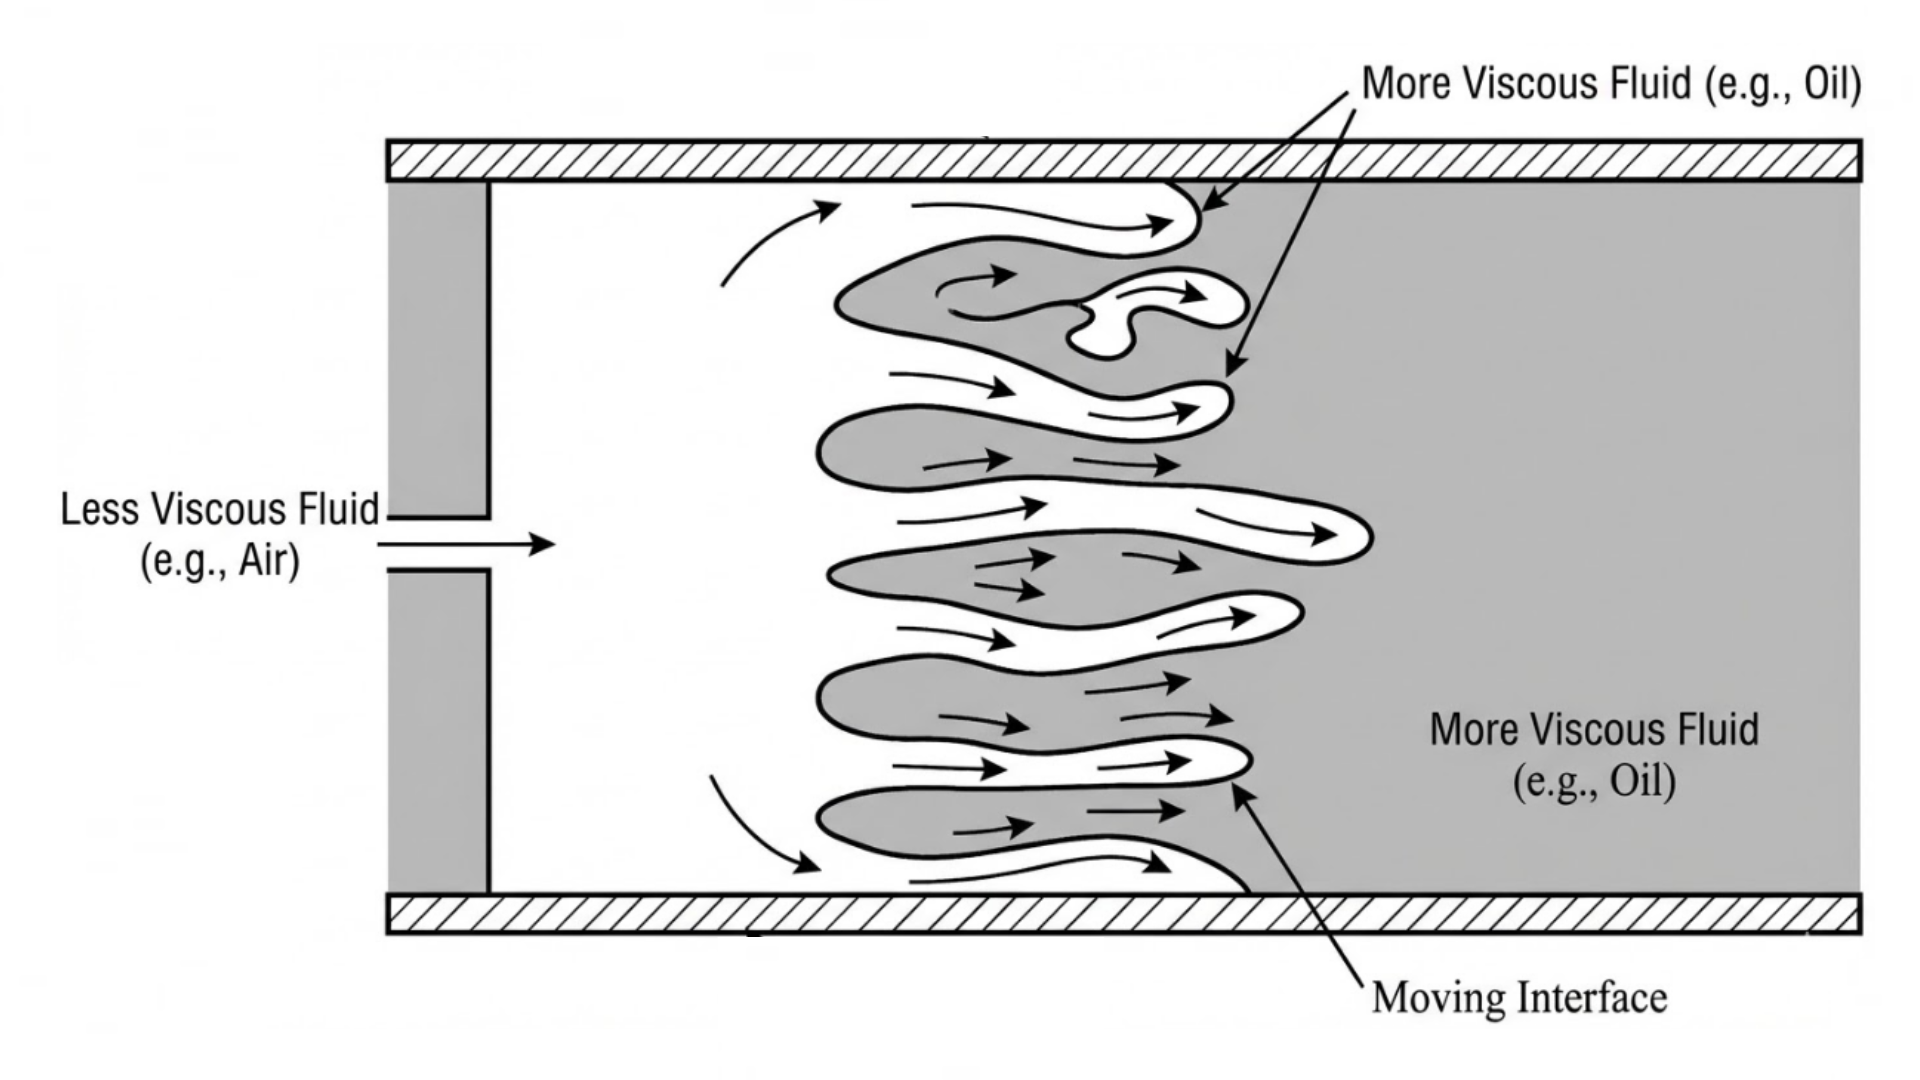
\includegraphics[width=0.8\linewidth]{figuras/introducao/fingering_example.png}
    \caption{Fingers patterns example}
    \label{fig:intro-saff-example}
\end{figure}


In the context of Enhanced Oil Recovery (EOR), the Saffman-Taylor instability acts as a  limiter to sweep efficiency. The propagation of viscous fingers leads to the premature breakthrough of the injected fluid at the production wells. Consequently, the water cut increases rapidly, leaving substantial volumes of bypassed, unrecoverable oil stranded within the reservoir matrix \cite{homsy1987viscous}. 

Various technological interventions have been developed to mitigate viscous fingering and improve the mobility ratio. Conventional chemical EOR strategies, such as polymer flooding, focus on increasing the apparent viscosity of the aqueous phase, thereby creating a more favorable mobility ratio and stabilizing the displacement front \cite{sheng2011modern}. More recent advancements involve the injection of foams, surfactants, and nanoparticle-stabilized emulsions (smart fluids) designed to alter interfacial tension and modify local rheology \cite{binks2002particles}. However, these approaches often face limitations regarding thermal degradation, mechanical shear degradation in the near-wellbore region, complex reservoir retention, and significant operational costs \cite{sorbie1991polymer, olajire2014review}.

To address these limitations, this study investigates a novel active-control mechanism: the application of magnetic fluids (ferrofluids) as the displacing phase. By exposing the injected magnetic fluid to an external magnetic field, an artificial body force (the Kelvin force) is induced at the fluid interface. Theoretical models and preliminary experiments demonstrate that a properly aligned magnetic field can counteract the hydrodynamic destabilization forces, effectively suppressing the Saffman-Taylor fingering \cite{jackson1993hydrodynamics, miranda1998radial}. 

Therefore, the primary objective of this thesis is the development and validation of a Computational Fluid Dynamics (CFD) simulation to model the multiphase displacement of oil by a magnetic fluid in a porous medium, supported by an analytical mathematical framework for theoretical validation. This computational framework will quantify the interfacial stabilization mechanisms and evaluate the sweep efficiency under varying magnetic field topologies and flow regimes.



%% FALAR O QUE É FLUIDO MAGNETICO 
%% QUANTIDADES DE PUBLICAÇÕES 
%% COMO AS PESSOAS ATACAM ESSES PROBLEMAS USUALMENTE
%% TEORIA PARA LEIGOS 
%% EXEMPLOS EXPERIMENTAIS DE SAFFMAN TAYLOR 
\section{Objectives}

\subsection{General Objective}
The primary objective of this thesis is to evaluate the suppression of the Saffman--Taylor instability in porous media during Enhanced Oil Recovery (EOR) processes using magnetic fluids. This is achieved through the development of an integrated framework comprising a rigorous analytical mathematical formulation and a Computational Fluid Dynamics (CFD) simulation.

\subsection{Specific Objectives}
To accomplish these goals, the following specific objectives are established:

\begin{itemize}
    \item \textbf{Analytical Formulation:} Formulate a Linear Stability Analysis (LSA) for the multiphase displacement involving a magnetic fluid under an external magnetic field, in order to derive the theoretical stability criteria and the perturbation dispersion relations.

    \item \textbf{Computational Modeling:} Develop and verify a multiphase CFD model based on the Cahn--Hilliard phase-field formulation coupled to a Lattice Boltzmann hydrodynamic solver, capable of simulating the nonlinear displacement of heavy oil by a magnetic fluid within a representative porous medium geometry.

    \item \textbf{Theoretical Validation:} Compare and validate the numerical predictions of the CFD model against the analytical thresholds established by the LSA, ensuring the physical accuracy of the computational framework prior to complex extrapolations.

    \item \textbf{Interfacial Dynamics Analysis:} Investigate the local fluid--fluid interaction, quantifying how varying magnetic field topologies physically alter the interfacial dynamics, either mitigating or potentially exacerbating finger growth.

    \item \textbf{Regime Mapping and EOR Evaluation:} Conduct a parametric study to map the flow regimes, comparing baseline conditions (conventional oil--water displacement) with magnetic fluid injection.
\end{itemize}
\include{capitulos/estado\_da\_arte}
\section{Theoretical Background}

This section establishes the theoretical foundation necessary to comprehend, analytically formulate, and numerically simulate the active control of viscous fingering in porous media. It will starts by examining fluid dynamics across different spatial scales, transitioning from the microscopic pore-level interactions to the macroscopic continuum descriptions governing flow in porous media. Subsequently, the physical principles of multiphase flow are addressed, with particular emphasis on the dynamic interactions between immiscible fluids, interfacial tension, and the resulting capillary phenomena. Building upon these interfacial concepts, the mathematical framework of Linear Stability Analysis (LSA) is introduced to rigorously describe the onset, growth, and governing parameters of the Saffman-Taylor instability.

Following the characterization of the instability, the physicochemical properties of magnetic fluids (ferrofluids) and the governing equations of magneto-hydrodynamics are presented. This provides the physical basis for how external magnetic fields exert stabilizing body forces (the Kelvin force) at the fluid-fluid interface. Finally, to bridge the gap between analytical stability criteria and complex, non-linear flow regimes, the theoretical basis of the Lattice Boltzmann Method (LBM) is detailed. Operating at a mesoscopic scale through the discrete Boltzmann equation, the LBM presents distinct advantages over traditional macroscopic Navier-Stokes solvers, particularly regarding the natural resolution of complex interfacial dynamics, phase separation, and the incorporation of external magnetic forces within the intricate geometries characteristic of porous matrixes.

\subsection{Flow in Porous Media}

\subsubsection{Micro-Scale Porous Media: The Stokes Limit}

At the microscopic scale, a porous medium is defined as a multiply connected domain $\Omega \subset \mathbb{R}^3$, partitioned into a fluid phase $\Omega_f$ and a stationary solid phase $\Omega_s$. The interface $\Gamma = \partial \Omega_f \cap \partial \Omega_s$ represents the complex topological boundary of the pore walls \cite{whitaker1999method}.

In this domain, the flow physics is strictly governed by the ratio of inertial forces to viscous forces \cite{batchelor1967introduction}.

\paragraph{Dimensional Analysis and the Stokes Regime}
The characterization of the flow regime relies on the Reynolds number defined at the pore scale. Let $\ell$ be the characteristic length scale (e.g., hydraulic diameter of a pore throat) and $U$ be the characteristic velocity scale within the pore.

\begin{equation}
    Re_\ell = \frac{\rho U \ell}{\mu}
\end{equation}

In micro-porous media (e.g., microfluidic networks, sedimentary rock matrices), $\ell$ is typically on the order of $10^{-6}$ to $10^{-4}$\,m. Consequently, even for moderate pressure gradients, $Re_\ell \ll 1$.

Applying the non-dimensionalization variables $\mathbf{x}^* = \mathbf{x}/\ell$, $\mathbf{u}^* = \mathbf{u}/U$, and $p^* = p \ell / (\mu U)$, the steady-state Navier-Stokes momentum equation becomes:

\begin{equation}
    Re_\ell (\mathbf{u}^* \cdot \nabla^*) \mathbf{u}^* = -\nabla^* p^* + {\nabla^*}^2 \mathbf{u}^*
\end{equation}

As $Re_\ell \to 0$, the inertial term on the left-hand side vanishes. The governing physics reduces to a balance between pressure gradients and viscous diffusion.

\paragraph{Governing Micro-Scale Equations}
The fluid motion in $\Omega_f$ is described by the Stokes equations (creeping flow) \cite{stokes1851effect}. The system is linear and instantaneous (time-independent):

\begin{itemize}
    \item \textbf{Momentum Balance:}
    \begin{equation}
        \nabla \cdot \boldsymbol{\sigma} = \mathbf{0} \implies \mu \nabla^2 \mathbf{u} - \nabla p = \mathbf{0}
    \end{equation}
    \item \textbf{Mass Conservation:}
    \begin{equation}
        \nabla \cdot \mathbf{u} = 0
    \end{equation}
\end{itemize}

Here, $\boldsymbol{\sigma}$ is the Newtonian stress tensor:
\begin{equation}
    \boldsymbol{\sigma} = -p\mathbf{I} + 2\mu \mathbf{D}
\end{equation}
where $\mathbf{D} = \frac{1}{2}(\nabla \mathbf{u} + (\nabla \mathbf{u})^T)$ is the rate-of-strain tensor.

\subsubsection{Meso-Scale Formulation: The Darcy-Brinkman Equation}

The transition from the micro-scale Stokes regime to the meso-scale continuum is achieved by averaging the governing equations over a Representative Elementary Volume, $V$. Let $V_f$ represent the fluid volume within $V$, and $A_{fs}$ represent the interfacial area between the fluid and the solid particles.

We define the superficial average velocity, $\mathbf{v} \equiv \langle \mathbf{u} \rangle$, as:
\begin{equation}
    \langle \mathbf{u} \rangle = \frac{1}{V} \int_{V_f} \mathbf{u} \, dV
\end{equation}

\paragraph{Volume Averaging of the Stokes Momentum Equation}
Starting with the micro-scale stationary Stokes momentum equation:
\begin{equation}
    -\nabla p + \mu \nabla^2 \mathbf{u} + \rho \mathbf{b} = 0
\end{equation}

We apply the averaging operator $\langle \cdot \rangle$ to each term. The critical mathematical tool required is the \textit{Spatial Averaging Theorem} (SAT), which allows us to commute the gradient and averaging operators \cite{whitaker1999method}:
\begin{equation}
    \langle \nabla \psi \rangle = \nabla \langle \psi \rangle + \frac{1}{V} \int_{A_{fs}} \psi \mathbf{n}_{fs} \, dA
\end{equation}
where $\mathbf{n}_{fs}$ is the unit normal vector pointing from the fluid to the solid.

\paragraph{Derivation of Terms}

\begin{enumerate}
    \item \textbf{Pressure Gradient:} Applying the SAT to $-\nabla p$:
    \begin{equation}
        -\langle \nabla p \rangle = -\nabla \langle p \rangle^f - \frac{1}{V} \int_{A_{fs}} p \mathbf{n}_{fs} \, dA
    \end{equation}
    Here, $\langle p \rangle^f$ is the intrinsic average pressure (pore pressure).

    \item \textbf{Viscous Term (Brinkman \& Drag):} Applying the SAT to $\mu \nabla^2 \mathbf{u}$ requires a second-order expansion. For high porosity media, we approximate \cite{brinkman1949calculation}:
    \begin{equation}
        \mu \langle \nabla^2 \mathbf{u} \rangle \approx \underbrace{\mu_{eff} \nabla^2 \mathbf{v}}_{\text{Brinkman Term}} + \underbrace{\frac{1}{V} \int_{A_{fs}} \mu (\nabla \mathbf{u}) \cdot \mathbf{n}_{fs} \, dA}_{\text{Shear Drag}}
    \end{equation}
    The first term represents the viscous diffusion of average momentum (important near boundaries), where $\mu_{eff}$ is the effective viscosity. The second term represents the viscous shear stress at the particle surfaces.

    \item \textbf{Body Force:} Assuming $\rho \mathbf{b}$ is constant over the domain:
    \begin{equation}
        \langle \rho \mathbf{b} \rangle = \phi \rho \mathbf{b} \approx \rho \mathbf{b} \quad (\text{per unit fluid volume})
    \end{equation}
\end{enumerate}

\paragraph{The Meso-Scale Equation}
Combining these averaged terms, we group the surface integrals (pressure drag and viscous shear) into a single body force vector $\mathbf{f}$:

\begin{equation}
    \mathbf{f} = \underbrace{-\frac{1}{V} \int_{A_{fs}} p \mathbf{n}_{fs} \, dA}_{\text{Form Drag}} + \underbrace{\frac{1}{V} \int_{A_{fs}} \mu (\nabla \mathbf{u}) \cdot \mathbf{n}_{fs} \, dA}_{\text{Viscous Drag}}
\end{equation}

This term $\mathbf{f}$ represents the \textbf{average resistance force exerted by the fixed particles on the fluid}. 

Substituting this back into the momentum balance yields the \textbf{Darcy-Brinkman equation}:

\begin{equation}
    -\nabla \langle p \rangle^f + \mu_{eff} \nabla^2 \mathbf{v} + \rho \mathbf{b} + \mathbf{f} = 0
\end{equation}

\subsubsection{Macroscopic Limits: From Brinkman to Darcy}

Having established the meso-scale momentum balance (Darcy-Brinkman), we can now formally construct Darcy's Law and determine the conditions under which each governing equation is valid. This process relies on the concept of \textbf{hydrodynamic screening}.

\paragraph{Construction of Darcy's Equation}
Starting from the generalized meso-scale equation derived previously (neglecting body forces $\mathbf{b}$ for brevity):

\begin{equation}
    -\nabla p + \mu_{eff} \nabla^2 \mathbf{v} - \frac{\mu}{K} \mathbf{v} = 0
\end{equation}

We perform a scaling analysis. Let $L_c$ be the characteristic length scale of the macroscopic flow variation (e.g., the size of the domain or the scale of pressure gradients). The differential terms scale as:

\begin{equation}
    \mu_{eff} \nabla^2 \mathbf{v} \sim \frac{\mu V}{L_c^2} \quad \text{and} \quad \frac{\mu}{K} \mathbf{v} \sim \frac{\mu V}{K}
\end{equation}

The ratio of the viscous stress term (Brinkman) to the drag term (Darcy) is defined by the dimensionless \textbf{Darcy number} ($Da$):

\begin{equation}
    \frac{\text{Viscous Stress}}{\text{Drag}} \sim \frac{\mu V / L_c^2}{\mu V / K} = \frac{K}{L_c^2} = Da
\end{equation}

In the limit where the macroscopic length scale is very large compared to the pore structure ($L_c^2 \gg K$, or $Da \to 0$), the viscous stress term $\mu_{eff} \nabla^2 \mathbf{v}$ becomes negligible. The equation asymptotically reduces to the algebraic balance known as \textbf{Darcy's Law}:

\begin{equation}
    -\nabla p - \frac{\mu}{K} \mathbf{v} = 0 \implies \mathbf{v} = -\frac{K}{\mu} \nabla p
\end{equation}

\subsubsection{Hydrodynamic Screening and Scale Selection}

The transition between these regimes is governed by the \textbf{Brinkman screening length}, defined as $\lambda = \sqrt{K}$.

\textbf{Physics of Screening:} In a porous medium, the solid matrix acts as a momentum sink. Shear waves generated at a boundary (e.g., a wall with a no-slip condition) cannot propagate indefinitely into the bulk fluid; they are "screened" or damped by the Darcy drag within a distance of order $O(\sqrt{K})$. 

This length scale allows us to select the appropriate governing equation based on the characteristic scale of the problem $L_c$ relative to the screening length.

\paragraph{Regime Selection Guide}

\begin{enumerate}
    \item \textbf{Micro-Scale Regime (Pore Level Physics)} \\
    \textit{Condition:} The length scale $L_c$ is comparable to the pore size $\ell_{pore}$ (or boundary layer $\delta$ inside a pore). \\
    At this scale, the medium is not a continuum. We must solve the flow around individual solid obstacles. Drag is not a volume force but a boundary integration result.
    \begin{equation}
        L_c \sim \ell_{pore} \quad \xrightarrow{} \quad -\nabla p + \mu \nabla^2 \mathbf{u} = 0 \quad (\text{Stokes Equation})
    \end{equation}

    \item \textbf{Meso-Scale / Transition Regime (Boundary Layers)} \\
    \textit{Condition:} The length scale $L_c$ is comparable to the screening length $\sqrt{K}$. \\
    This occurs near confining walls or interfaces between porous and pure fluid regions. The boundary layer thickness $\delta$ is of order $\sqrt{K}$. Here, both viscous diffusion (shear) and Darcy drag are equally important.
    \begin{equation}
        L_c \sim \sqrt{K} \quad \xrightarrow{} \quad -\nabla p + \mu_{eff} \nabla^2 \mathbf{v} - \frac{\mu}{K} \mathbf{v} = 0 \quad (\text{Darcy-Brinkman})
    \end{equation}

    \item \textbf{Macro-Scale Regime (Bulk Porous Flow)} \\
    \textit{Condition:} The length scale $L_c$ is much larger than the screening length. \\
    The flow perceives the medium as a homogeneous resistance. Viscous shear is screened out, and the velocity is determined locally by the pressure gradient.
    \begin{equation}
        L_c \gg \sqrt{K} \quad \xrightarrow{} \quad -\nabla p - \frac{\mu}{K} \mathbf{v} = 0 \quad (\text{Darcy Equation})
    \end{equation}
\end{enumerate}

\subsubsection{Experimental Analogue: The Hele-Shaw Cell}

To facilitate experimental validation and visualize the hydrodynamic instabilities discussed (e.g., Saffman-Taylor), we utilize the Hele-Shaw cell configuration. This setup serves as a rigorous two-dimensional analogue to Darcy flow in porous media \cite{saffman1958penetration}.

\paragraph{Geometric Setup and Governing Equations}
Consider a fluid confined between two parallel plates separated by a small gap of thickness $h$, with lateral dimensions $L$ and $b$ such that $h \ll L, b$ \cite{batchelor1967introduction}. The flow is driven by a pressure gradient $\nabla P$ in the $(x, z)$ plane.

Under the conditions of low Reynolds number ($Re = \rho \bar{U} h / \mu \ll 1$) and high aspect ratio (Lubrication Approximation), the inertial terms in the Navier-Stokes equations are negligible \cite{bear1972dynamics}. The momentum balance reduces to a balance between the pressure gradient and the viscous shear across the gap thickness ($y$-direction):

\begin{equation}
    \frac{\partial P}{\partial x} = \mu \frac{\partial^2 u}{\partial y^2}, \quad \frac{\partial P}{\partial z} = \mu \frac{\partial^2 w}{\partial y^2}
\end{equation}
where $u$ and $w$ are the velocity components in the $x$ and $z$ directions, respectively. Note that $\partial P / \partial y \approx 0$.

\paragraph{Velocity Profile and Averaging}
We apply no-slip boundary conditions at the walls ($y=0$ and $y=h$):
\begin{equation}
    u(0) = u(h) = 0
\end{equation}

Integrating the momentum equation twice with respect to $y$, we obtain the parabolic velocity profile characteristic of Poiseuille flow \cite{batchelor1967introduction}:

\begin{equation}
    \mathbf{u}(y) = \frac{1}{2\mu} \nabla P (y^2 - hy)
\end{equation}

To establish the analogy with Darcy's Law, we calculate the gap-averaged velocity $\bar{\mathbf{u}}$ (or superficial velocity). This is obtained by integrating the profile over the gap height $h$:

\begin{equation}
    \bar{\mathbf{u}} = \frac{1}{h} \int_0^h \mathbf{u}(y) \, dy = \frac{\nabla P}{2\mu h} \int_0^h (y^2 - hy) \, dy
\end{equation}

Evaluating the definite integral $\int_0^h (y^2 - hy) dy = [\frac{y^3}{3} - \frac{hy^2}{2}]_0^h = -\frac{h^3}{6}$:

\begin{equation}
    \bar{\mathbf{u}} = \frac{\nabla P}{2\mu h} \left( -\frac{h^3}{6} \right) = -\frac{h^2}{12\mu} \nabla P
\end{equation}

\paragraph{Effective Permeability Definition}
Comparing this result with the standard Darcy's Law for a porous medium, $\bar{\mathbf{u}} = -\frac{K}{\mu} \nabla P$, we identify the effective permeability $K$ of the Hele-Shaw cell \cite{bear1972dynamics}:

\begin{equation}
    K_{HS} = \frac{h^2}{12}
\end{equation}

This relationship demonstrates that the permeability in this experimental setup is strictly determined by the gap width $h$. By controlling $h$, we can precisely tune the "permeability" of the medium in the lab, enabling accurate scaling of instability phenomena such as viscous fingering.

\subsection{Multiphase Flow in Porous Media}

In the context of Enhanced Oil Recovery (EOR) and the specific problem of viscous fingering, the porous medium is rarely saturated by a single fluid. The simultaneous flow of two or more immiscible fluids (e.g., heavy oil and an aqueous magnetic fluid) requires an extension of the macroscopic equations derived for single-phase flow.

\subsubsection{Phase Saturation and the Extended Darcy's Law}

When multiple immiscible phases occupy the void space of a porous medium, the volume fraction of the pore space occupied by a specific phase $\alpha$ is defined as its saturation, $S_\alpha$:
\begin{equation}
    S_\alpha = \frac{V_\alpha}{V_p}
\end{equation}
where $V_\alpha$ is the volume of phase $\alpha$ and $V_p$ is the total pore volume. By definition, for a fully saturated medium containing $n$ phases, $\sum_{i=1}^n S_i = 1$.

The presence of a second phase introduces capillary forces and reduces the available cross-sectional area for the flow of the first phase. Consequently, the absolute permeability $K$, which is strictly a geometric property of the solid matrix, is no longer sufficient to describe the flow conductance. We must introduce the concept of \textbf{effective permeability}, $K_\alpha$, which is the permeability of the medium to phase $\alpha$ at a given saturation $S_\alpha$.

The phenomenological extension of Darcy's Law for a multiphase system postulates that the superficial velocity of phase $\alpha$, $\mathbf{v}_\alpha$, is driven by its own phase pressure gradient $\nabla p_\alpha$:
\begin{equation}
    \mathbf{v}_\alpha = -\frac{K_\alpha}{\mu_\alpha} (\nabla p_\alpha - \rho_\alpha \mathbf{g})
\end{equation}

\subsubsection{Relative Permeability}

To normalize the flow equations, the effective permeability is expressed as the product of the absolute permeability $K$ and a dimensionless scaling factor known as the \textbf{relative permeability}, $k_{r\alpha}$:
\begin{equation}
    K_\alpha = K k_{r\alpha} \quad \text{where} \quad 0 \leq k_{r\alpha} \leq 1
\end{equation}

Unlike absolute permeability, $k_{r\alpha}$ is not solely a property of the rock. It is a highly non-linear, phenomenological function that depends primarily on the phase saturation ($k_{r\alpha} = f(S_\alpha)$), but also on the pore-size distribution, wettability of the solid matrix, and the flow history (hysteresis). The relative permeability accounts for the momentum dissipation at the fluid-fluid interfaces and the tortuous pathways forced upon one phase by the presence of the other.

Substituting into the extended Darcy's equation (neglecting gravity):
\begin{equation}
    \mathbf{v}_\alpha = -\frac{K k_{r\alpha}}{\mu_\alpha} \nabla p_\alpha
\end{equation}

\subsubsection{Phase Mobility and the Mobility Ratio}

The dynamic capacity of a specific phase to flow through the porous medium under a given pressure gradient is quantified by its \textbf{mobility}, $\lambda_\alpha$. It couples the rock-fluid interaction parameter ($k_{r\alpha}$) with the intrinsic fluid property (dynamic viscosity $\mu_\alpha$):
\begin{equation}
    \lambda_\alpha = \frac{K k_{r\alpha}}{\mu_\alpha} \implies \mathbf{v}_\alpha = -\lambda_\alpha \nabla p_\alpha
\end{equation}

In a displacement process, such as the injection of a magnetic fluid (aqueous phase, subscript $w$) to displace heavy oil (subscript $o$), the hydrodynamic stability of the displacement front is governed by the \textbf{Mobility Ratio}, $M$. It is defined as the ratio of the mobility of the displacing fluid behind the front to the mobility of the displaced fluid ahead of the front:
\begin{equation}
    M = \frac{\lambda_w}{\lambda_o} = \frac{k_{rw} / \mu_w}{k_{ro} / \mu_o} = \frac{k_{rw} \mu_o}{k_{ro} \mu_w}
\end{equation}

The mobility ratio is the critical dimensionless parameter determining macroscopic sweep efficiency:
\begin{itemize}
    \item \textbf{$M \leq 1$ (Favorable Displacement):} The displaced fluid is more mobile than the injected fluid. The pressure field is stable, and the displacement front tends to remain planar and uniform.
    \item \textbf{$M > 1$ (Adverse Displacement):} The injected fluid has higher mobility (e.g., injecting low-viscosity water to displace high-viscosity oil). The displacement front becomes inherently unstable to infinitesimally small perturbations.
\end{itemize}

This adverse mobility condition ($M>1$) is the fundamental physical trigger for the hydrodynamic instability known as viscous fingering, which necessitates the introduction of active control mechanisms such as magnetic fluids.

\subsection{Phase-Field Modeling: The Cahn-Hilliard Equation}

The mobility ratio criterion established above identifies when an immiscible displacement becomes hydrodynamically unstable, but it does not by itself prescribe how the fluid-fluid interface is to be represented and tracked through space and time. In a classical sharp-interface formulation, the interface $\Gamma(t)$ is treated as a co-dimension-one manifold whose evolution is governed by free-boundary kinematic and dynamic conditions (continuity of normal velocity and a Laplace-type pressure jump set by the local curvature and the surface tension). Solving such a formulation in geometries as topologically complex as a porous matrix, where the interface routinely undergoes pinch-off, coalescence, and fingering events, is analytically intractable and numerically requires explicit reconstruction of $\Gamma(t)$ at every time step.

To circumvent these difficulties we adopt a diffuse-interface (phase-field) description, in which the interface is regularised over a finite thickness $W$ by introducing a conserved scalar order parameter $\phi(\mathbf{x}, t)$ that varies smoothly between two bulk equilibrium values:
\begin{equation}
    \phi(\mathbf{x}, t) = \begin{cases}
        +1 & \text{invading (magnetic) phase}, \\
        -1 & \text{resident (oleic) phase}, \\
        \in (-1, +1) & \text{interfacial region}.
    \end{cases}
\end{equation}
The geometric interface is then implicitly defined as the level set $\{\mathbf{x} : \phi(\mathbf{x}, t) = 0\}$, and topological events are handled automatically without remeshing or geometric reconstruction.

\subsubsection{Ginzburg-Landau Free-Energy Functional}

The thermodynamics of the two-phase system is encoded by the Ginzburg-Landau free-energy functional \cite{cahn1958free}:
\begin{equation}
    \mathcal{F}[\phi] = \int_{\Omega} \left[ \underbrace{\beta\,(\phi^2 - 1)^2}_{\text{double-well (bulk)}} + \underbrace{\tfrac{\kappa}{2}\,|\nabla \phi|^2}_{\text{gradient penalty}} \right] d\Omega.
\end{equation}
The bulk term $\beta(\phi^2 - 1)^2$ is a symmetric double-well potential with degenerate minima at $\phi = \pm 1$, expressing the thermodynamic preference of the system for pure phases over mixed states. The gradient term $(\kappa/2)|\nabla \phi|^2$ penalises sharp variations of $\phi$ and is responsible for the finite interface thickness; without it, minimisation of $\mathcal{F}$ would drive the interface towards a singular discontinuity. The two parameters $\beta$ and $\kappa$ are independent, with positive units, and jointly control the macroscopic interfacial properties of the diffuse model.

\subsubsection{Chemical Potential and the Cahn-Hilliard Equation}

The chemical potential associated with the order parameter is defined as the functional derivative of $\mathcal{F}$:
\begin{equation}
    \mu_c = \frac{\delta \mathcal{F}}{\delta \phi} = 4\beta\,\phi(\phi^2 - 1) - \kappa\,\nabla^2 \phi.
\end{equation}
For an incompressible two-phase flow with velocity field $\mathbf{u}$, the conservative evolution of the order parameter is governed by the advective Cahn-Hilliard equation \cite{cahn1958free}:
\begin{equation}
    \frac{\partial \phi}{\partial t} + \mathbf{u} \cdot \nabla \phi = M\,\nabla^2 \mu_c,
\end{equation}
where $M$ is the mobility coefficient (with units of $L^2 T^{-1}$ per unit chemical potential). The advective term on the left transports the phase distribution by the hydrodynamic field, while the right-hand side drives the diffusive relaxation of $\phi$ towards the local minimisers of $\mathcal{F}$, counteracting the numerical thickening of the interface caused by advection. Because the right-hand side can be written as the divergence of a flux,
\begin{equation}
    M\,\nabla^2 \mu_c = \nabla \cdot \left(M \nabla \mu_c\right) \implies \mathbf{J} = \phi\mathbf{u} - M\nabla \mu_c, \qquad \frac{\partial \phi}{\partial t} = -\nabla \cdot \mathbf{J},
\end{equation}
the Cahn-Hilliard equation conserves the total amount of each phase exactly in closed domains:
\begin{equation}
    \frac{d}{dt} \int_{\Omega} \phi\, d\Omega = -\oint_{\partial \Omega} \mathbf{J} \cdot \hat{\mathbf{n}}\, dS.
\end{equation}
This conservation property distinguishes the Cahn-Hilliard model (fourth-order in $\phi$, conservative) from the Allen-Cahn model (second-order, non-conservative) and is essential for long-time simulations of immiscible displacement, where loss of mass would bias the measured fingering growth rates and saturation profiles.

\subsubsection{Equilibrium Profile and Interfacial Tension}

For a stationary planar interface aligned with the $z = 0$ plane (no advection, $\partial_t \phi = 0$), the Cahn-Hilliard equation reduces to $\nabla^2 \mu_c = 0$ subject to $\phi(\pm \infty) = \pm 1$ and $\mu_c(\pm\infty) = 0$, yielding $\mu_c \equiv 0$ throughout the domain. The chemical-potential definition then becomes a nonlinear ordinary differential equation,
\begin{equation}
    4\beta\,\phi(\phi^2 - 1) - \kappa\,\frac{d^2 \phi}{dz^2} = 0,
\end{equation}
whose physical solution is the hyperbolic-tangent profile
\begin{equation}
    \phi_{eq}(z) = \tanh\!\left( \frac{z\sqrt{2}}{W} \right), \qquad W = \sqrt{\frac{\kappa}{2\beta}},
\end{equation}
where $W$ is the characteristic interface thickness. Integrating the gradient-energy density across the interface yields the effective interfacial tension associated with the diffuse-interface model:
\begin{equation}
    \sigma = \int_{-\infty}^{+\infty} \kappa \left(\frac{d\phi_{eq}}{dz}\right)^{\!2} dz = \frac{2\sqrt{2}}{3}\sqrt{\kappa\,\beta}.
\end{equation}
Inverting these two algebraic identities permits independent calibration: given target physical values of $\sigma$ and $W$, the model parameters are recovered as $\beta = 3\sqrt{2}\,\sigma/(4W)$ and $\kappa = 3\sqrt{2}\,\sigma\,W/4$. This separation of the two macroscopic interface properties into two independent model parameters is one of the key reasons for choosing the Cahn-Hilliard formulation as the multiphase backbone in this work.

\subsubsection{Coupling to the Momentum Equation: Korteweg Stress}

To close the multiphase Navier-Stokes/Darcy-Brinkman momentum balance, the diffuse-interface model must supply the capillary body force. By Noether's theorem applied to translations of the free energy $\mathcal{F}$, the surface-tension contribution can be written in compact form as the Korteweg stress, whose body-force representation is
\begin{equation}
    \mathbf{F}_s = \mu_c\,\nabla \phi.
\end{equation}
Outside the diffuse interfacial layer $\nabla \phi \approx 0$ and $\mathbf{F}_s$ vanishes identically; within the layer the force is non-zero and acts along the local interface normal, with a magnitude that reproduces, in the sharp-interface limit ($W \to 0$ at fixed $\sigma$), the standard capillary forcing $\sigma\,\kappa_c\,\hat{\mathbf{n}}\,\delta_{\Gamma}$, where $\kappa_c$ is the local mean curvature. In this manner the Cahn-Hilliard equation supplies, in a single scalar field $\phi$, three quantities required by the full multiphase formulation: the implicit geometric tracking of the interface (level set $\phi = 0$), the conservation of phase volumes (divergence form of the flux $\mathbf{J}$), and the capillary forcing $\mathbf{F}_s$ to be inserted into the momentum equation. The numerical implementation of this coupling within the Lattice Boltzmann framework is detailed in the next chapter.




















\subsection{Magnetic Fluids: Fundamentals and Properties}

To effectively control hydrodynamic instabilities such as viscous fingering, this study employs magnetic fluids as the active displacing phase. Magnetic fluids, commonly referred to as ferrofluids, are a unique class of smart fluids that exhibit magnetic properties. As described by Rosensweig \cite{rosensweig1985ferrohydrodynamics}, these fluids are not true homogenous solutions, but rather highly stable colloidal suspensions.

A typical ferrofluid consists of three primary components:
\begin{enumerate}
    \item \textbf{Magnetic Nanoparticles:} Single-domain particles, typically composed of magnetite ($\text{Fe}_3\text{O}_4$) or maghemite ($\gamma\text{-Fe}_2\text{O}_3$), with diameters on the order of $10$ nanometers.
    \item \textbf{Carrier Liquid:} The continuous non-magnetic fluid phase in which the particles are dispersed, which can be aqueous or organic (e.g., water, kerosene, or synthetic oils).
    \item \textbf{Surfactant Coating:} To prevent the agglomeration of the nanoparticles due to strong short-range van der Waals attractive forces and magnetic dipole-dipole interactions, the particles are coated with a layer of long-chain surfactant molecules (steric repulsion) or stabilized via electrostatic charge.
\end{enumerate}

A defining characteristic of these stable suspensions is their superparamagnetic behavior. In the absence of an external magnetic field, the magnetic moments of the individual nanoparticles are randomly oriented due to thermal agitation, resulting in a net macroscopic magnetization of zero. Upon the application of an external magnetic field, the particle moments rapidly align with the field lines. 

The mathematical validity of treating this biphasic suspension as a homogeneous, single-phase continuum in macroscopic flow equations relies on two critical scale separations: spatial and temporal \cite{rosensweig1985ferrohydrodynamics}. 

Spatially, let $d_p$ be the average diameter of the coated magnetic nanoparticles and $D_p$ be the characteristic length scale of the porous matrix (e.g., the pore throat diameter). As established by Rosensweig \cite{rosensweig1985ferrohydrodynamics}, typical ferrofluid nanoparticles possess $d_p \sim \mathcal{O}(10^{-8} \text{ m})$. Conversely, extensive petrophysical characterizations by Dullien \cite{dullien1992porous} indicate that standard reservoir rock pore throats are on the order of $D_p \sim \mathcal{O}(10^{-5} \text{ to } 10^{-4} \text{ m})$. The spatial scale ratio is therefore:
\begin{equation}
    \epsilon = \frac{d_p}{D_p} \sim 10^{-4} \ll 1
\end{equation}
Because $\epsilon \ll 1$, the discrete nature of the nanoparticles is negligible, and the fluid perfectly conforms to the continuum hypothesis required for the Navier-Stokes and Darcy formulations.

Temporally, the fluid's response to dynamic flow conditions and changing magnetic fields is governed by its magnetic relaxation time, $\tau$. In ferrofluids, relaxation occurs via two parallel mechanisms formulated by Rosensweig \cite{rosensweig1985ferrohydrodynamics}: the physical rotation of the particle within the fluid (Brownian relaxation, $\tau_B$) and the internal rotation of the magnetic moment within the particle's crystalline lattice (Néel relaxation, $\tau_N$). The effective relaxation time is dominated by the faster of the two processes:
\begin{equation}
    \tau = \left( \frac{1}{\tau_B} + \frac{1}{\tau_N} \right)^{-1}
\end{equation}
For $10$ nm magnetite particles, $\tau$ is extremely short, typically $\mathcal{O}(10^{-6} \text{ s})$. Conversely, the characteristic hydrodynamic time scale of the flow in the porous medium is $t_f = D_p / U$, which is generally $\mathcal{O}(10^{-2} \text{ to } 1 \text{ s})$. 

This temporal separation is rigorously quantified by the dimensionless Deborah number ($De$), a standard rheological metric defined as the ratio of the fluid's relaxation time to the characteristic time of the flow:
\begin{equation}
    De = \frac{\tau}{t_f} \ll 1
\end{equation}
Because $De$ is asymptotically close to zero, the magnetic moments adjust to local field variations and flow vorticity instantaneously relative to the fluid motion. This mathematical condition ensures that the ferrofluid lacks viscoelastic memory, behaving as a purely viscous Newtonian fluid, and that its macroscopic magnetization $\mathbf{M}$ is always in collinear thermodynamic equilibrium with the applied field $\mathbf{H}$ (i.e., $\mathbf{M} = \chi \mathbf{H}$). Consequently, these spatial and temporal conditions provide the exact physical foundation to dynamically control the fluid interface in porous media via macroscopic external fields.

\subsection{The Kelvin Force and Effective Magnetic Pressure}

The physical coupling between the external magnetic field and the fluid flow within the porous medium occurs through a volumetric body force known as the Kelvin force. Because the ferrofluid is electrically non-conductive, the standard Lorentz force (associated with moving free charges) is completely absent. The macroscopic magnetic force density $\mathbf{f}_m$ acting on a magnetizable fluid is defined as:
\begin{equation}
    \mathbf{f}_m = \mu_0 (\mathbf{M} \cdot \nabla)\mathbf{H}
\end{equation}
where $\mathbf{H}$ is the macroscopic magnetic field intensity, $\mathbf{M}$ is the fluid's magnetization, and $\mu_0$ is the vacuum magnetic permeability.

Under the condition of a superparamagnetic fluid in thermodynamic equilibrium, the magnetization is collinear and proportional to the magnetic field, such that $\mathbf{M} = \chi \mathbf{H}$, where $\chi$ is the magnetic susceptibility. Applying vector calculus identities, and given that the magnetic field is irrotational in the absence of free currents ($\nabla \times \mathbf{H} = \mathbf{0}$), this force can be analytically rewritten as the gradient of the squared magnetic field intensity:
\begin{equation}
    \mathbf{f}_m = \frac{1}{2} \mu_0 \chi \nabla H^2
\end{equation}

As extensively detailed in the comprehensive review of ferrohydrodynamics by Gontijo and Cunha \cite{gontijo_cunha_review}, because this Kelvin force is strictly conservative ($\nabla \times \mathbf{f}_m = \mathbf{0}$), it acts mathematically as an artificial pressure gradient. Incorporating this volumetric body force into the macroscopic Darcy's law yields the coupled momentum equation for the magnetic phase:
\begin{equation}
    \frac{\eta}{K} \mathbf{v} = -\nabla p + \nabla \left( \frac{1}{2} \mu_0 \chi H^2 \right)
\end{equation}


Because both the thermodynamic pressure gradient and the Kelvin force are gradients of scalar fields, the magnetic force can be analytically absorbed into a modified, or effective, pressure $p^*$:
\begin{equation}
    p^* = p - \frac{1}{2} \mu_0 \chi H^2 \implies \frac{\eta}{K} \mathbf{v} = -\nabla p^*
\end{equation}

This fundamental mathematical arrangement demonstrates that the external magnetic field locally modulates the pressure field of the fluid. Furthermore, since the velocity vector $\mathbf{v}$ is strictly proportional to the gradient of this effective pressure ($p^*$), the velocity field remains irrotational. This property permits the mathematical definition of a velocity potential $\phi$ such that $\mathbf{v} = \nabla \phi$, fulfilling Laplace's equation in incompressible domains. The structural equivalence between the Kelvin force and a pressure drop establishes the theoretical mechanism by which the external magnetic field can be precisely manipulated to alter local velocity gradients at the interface, counteracting viscous fingering.

%% ter cuidado de justificar paramagnetismo com deborah
%% equação evolutiva da relaxação da magnetização 
\include{capitulos/regime\_linear\_lsa}
\include{capitulos/lbm\_teoria}
\section{Results}

Having validated the hydrodynamic (Poiseuille) and porous (Darcy--Brinkman) branches of the kernel in the previous section, this section assesses the central physical claim of the work: that the lattice-Boltzmann solver reproduces the \emph{growth rate} of an interfacial perturbation predicted by the linear stability analysis (LSA) of Section~\ref{sec:lsa}. The comparison is performed in the asymptotic linear regime, where the interface amplitude is small enough that the dispersion relation~\eqref{eq:dispersion_nondim} holds, and is carried out for a sweep of phase-field resolutions and initial amplitudes in order to characterise the numerical conditions under which the analytical prediction is recovered.

\subsection{Numerical Extraction of the Interfacial Growth Rate}
\label{sec:growth_rate_method}

The quantity to be compared with the LSA is the temporal growth rate $s$ of a single sinusoidal interface mode of order $m$. Its extraction from the raw simulation snapshots follows a four-stage pipeline (implemented in \texttt{post\_process/valida\_lsa.py} and batched over all cases by \texttt{post\_process/extrai\_resultados\_lsa.py}).

\paragraph{(i) Sub-cell interface localisation.} For each saved snapshot, the interface position $x(y)$ is located row by row as the zero crossing of the phase field $\phi$. Rather than snapping to the nearest cell, the crossing is resolved with sub-cell accuracy by linear interpolation between the two straddling nodes,
\begin{equation}
    x(y) = x_l + \frac{\phi_l}{\phi_l - \phi_r}, \qquad \phi_l = \phi(y,x_l) > 0,\ \ \phi_r = \phi(y,x_{l+1}) < 0,
\end{equation}
which suppresses the staircase quantisation error that would otherwise contaminate the amplitude of low-amplitude modes.

\paragraph{(ii) Modal amplitude by Fourier projection.} The amplitude of the target mode $m$ is obtained by projecting the interface contour onto the corresponding harmonic, rather than by a peak-to-valley ($\max-\min$) measurement. This isolates the mode of interest from numerical noise and from spurious higher harmonics:
\begin{equation}
    A_m(t) = \frac{2}{N_y}\left| \sum_{y=0}^{N_y-1} x(y,t)\,e^{-2\pi i\,m\,y/N_y} \right|.
    \label{eq:fourier_amplitude}
\end{equation}

\paragraph{(iii) Identification of the linear window.} Linear theory predicts pure exponential growth, $A_m(t) = A_0\,e^{s t}$, only during a finite interval bounded below by the initial diffusive relaxation of the interface and above by the onset of nonlinear saturation (finger formation). To select this interval objectively, the instantaneous growth rate $s_{\mathrm{loc}}(t) = \mathrm{d}\ln A_m/\mathrm{d}t$ is computed by a local linear regression over a sliding $\pm k$-point window, and the fitting interval $[t_0,t_1]$ is taken as the contiguous plateau around the peak of $s_{\mathrm{loc}}$ where $|s_{\mathrm{loc}} - s_{\mathrm{peak}}|/s_{\mathrm{peak}} \le \mathrm{tol}$, with the tolerance relaxed in steps ($4\% \to 20\%$) until at least six points are captured. This removes operator bias from the choice of fitting window.

\paragraph{(iv) Fit and non-dimensionalisation.} The numerical growth rate $s_{\mathrm{num}}$ is the slope of a least-squares fit of $\ln A_m$ against $t$ over the linear window. It is rendered dimensionless using the same scaling as the LSA, namely the domain height $L_{\mathrm{ref}} = N_y$ as the length scale and the inlet velocity $U = U_{\mathrm{in}}$ as the velocity scale:
\begin{equation}
    \zeta_{\mathrm{num}} = s_{\mathrm{num}}\,\frac{L_{\mathrm{ref}}}{U}, \qquad \alpha = k\,L_{\mathrm{ref}} = 2\pi m .
    \label{eq:zeta_num}
\end{equation}
The analytical counterpart $\zeta_{\mathrm{ana}}$ is evaluated directly from the dimensionless dispersion relation~\eqref{eq:dispersion_nondim} at the simulated wavenumber $\alpha = 2\pi m$, and the agreement is quantified by the relative error $\varepsilon = |s_{\mathrm{num}} - s_{\mathrm{ana}}|/|s_{\mathrm{ana}}|$.


\subsection{Comparison with the Linear Dispersion Relation}
\label{sec:lsa_comparison}

Table~\ref{tab:comparacao_lsa} reports, for every case, the numerically extracted growth rate alongside the analytical prediction. Because the dimensionless target $\zeta_{\mathrm{ana}} \approx 3.745$ is grid-independent, the dimensionless rate $\zeta$ is the natural basis for comparison; the dimensional $s$ differs between groups only through the scaling $s = \zeta\,U/N_y$.

\begin{table}[!ht]
\centering
\caption{Comparison between the numerically extracted interfacial growth rate (LBM) and the linear stability prediction (LSA, Eq.~\eqref{eq:dispersion_nondim}), for $m=1$, $M=4$, $\mathrm{Da}\approx1.25\times10^{-4}$, $\mathrm{Ca}=0.25$. Here $W$ is the diffuse-interface width and $A_0$ the initial amplitude (lattice units), $k\xi = 2\pi m W/N_y$ is the phase-field resolution number, $\zeta = s\,N_y/U$ is the dimensionless growth rate, $\varepsilon$ is the relative error on $s$, and $R^2$ is the goodness of fit of the log-linear regression over the identified linear window.}
\label{tab:comparacao_lsa}
\small
\begin{tabular}{l c c c c c c c}
\hline
Case & $W$ & $A_0$ & $k\xi$ & $\zeta_{\mathrm{num}}$ & $\zeta_{\mathrm{ana}}$ & $\varepsilon$ (\%) & $R^2$ \\
\hline
\multicolumn{8}{l}{\textit{Group AB --- interface thickness sweep ($N_y = 800$)}}\\
AB, $W{=}1$        & 1 & 0.20 & 0.0079 & 5.391 & 3.745 & 43.9 & 0.749 \\
AB, $W{=}2$        & 2 & 0.40 & 0.0157 & 3.668 & 3.745 &  2.1 & 0.994 \\
AB, $W{=}4$        & 4 & 0.80 & 0.0314 & 3.530 & 3.745 &  5.7 & 1.000 \\
\hline
\multicolumn{8}{l}{\textit{Group AC --- thickness $\times$ amplitude cross-sweep ($N_y = 1024$)}}\\
AC, $W{=}3$, $A_0{=}W/10$ & 3 & 0.30 & 0.0184 & 3.914 & 3.745 &  4.5 & 0.953 \\
AC, $W{=}3$, $A_0{=}W/5$  & 3 & 0.60 & 0.0184 & 3.502 & 3.745 &  6.5 & 1.000 \\
AC, $W{=}4$, $A_0{=}W/10$ & 4 & 0.40 & 0.0245 & 3.661 & 3.745 &  2.2 & 0.998 \\
AC, $W{=}4$, $A_0{=}W/5$  & 4 & 0.80 & 0.0245 & 3.493 & 3.745 &  6.7 & 1.000 \\
\hline
\multicolumn{8}{l}{\textit{Group AD --- robustness variants ($N_y = 1024$, $W = 3$)}}\\
AD, \texttt{Mlow}     & 3 & 0.30 & 0.0184 & 3.875 & 3.745 &  3.5 & 0.958 \\
AD, \texttt{linvisc}  & 3 & 0.30 & 0.0184 & 3.903 & 3.745 &  4.2 & 0.952 \\
AD, $A_0{=}W/20$      & 3 & 0.15 & 0.0184 & 5.012 & 3.745 & 33.8 & 0.731 \\
\hline
\end{tabular}
\end{table}

Figure~\ref{fig:comparacao_lsa} illustrates the comparison for a representative well-resolved case. The left panel shows the measured amplitude $A_m(t)$ on a semi-logarithmic scale, the fitted exponential, and the analytical slope anchored at the first valid point; the shaded band marks the automatically identified linear window. The right panel places the numerical and analytical rates on the analytical dispersion curve $\zeta(\alpha)$ at the simulated wavenumber $\alpha = 2\pi$.

\begin{figure}[!ht]
    \centering
    \includegraphics[width=0.92\linewidth]{figuras/validacao_lbm/comparacao_lsa_W4amp10.png}
    \caption{Representative LBM--LSA comparison (Group AC, $W=4$, $A_0 = W/10$). \textbf{Left:} interfacial amplitude $A_m(t)$ extracted by Fourier projection (markers), the exponential fit over the identified linear window (solid), and the analytical growth (dashed). \textbf{Right:} the dimensionless dispersion relation $\zeta(\alpha)$ with the numerical ($\zeta_{\mathrm{num}}$) and analytical ($\zeta_{\mathrm{ana}}$) rates marked at $\alpha = 2\pi$.}
    \label{fig:comparacao_lsa}
\end{figure}

\subsection{Error Analysis and Convergence}
\label{sec:error_analysis}

Discarding the two pathological configurations identified below, the LBM recovers the analytical growth rate with a relative error between $2.1\%$ and $6.7\%$ (mean $\approx 4.4\%$), with log-linear fits of quality $R^2 \ge 0.95$ and typically $R^2 > 0.99$. Given that the measured quantity is an exponential \emph{rate} --- the logarithmic derivative of an amplitude that itself must be reconstructed from a diffuse interface --- this level of agreement constitutes a quantitative validation of the instability physics encoded in the solver, not merely a qualitative one.

\paragraph{Interface thickness (Nyquist floor).} Group AB exposes a sharp lower bound on the admissible interface width. The $W=1$ case overpredicts the rate by $43.9\%$ with a poor fit ($R^2 = 0.75$): a single-cell diffuse interface violates the Nyquist criterion for resolving the phase-field gradients on the D2Q9 lattice, so the surface-tension stress is corrupted by spurious currents and the interface advects faster than physical. Increasing the thickness to $W=2$ collapses the error to $2.1\%$, and $W=4$ yields a near-perfect fit ($R^2 = 1.000$) at $5.7\%$. A diffuse interface of at least two lattice units is therefore a prerequisite for quantitative agreement; below it, the comparison is dominated by discretisation artefacts rather than by the modelled physics.

\paragraph{Initial amplitude (signal-to-noise floor).} The amplitude sweeps reveal a competing constraint at the opposite extreme. Reducing the initial amplitude sharpens adherence to the linear regime --- the $A_0 = W/10$ cases sit slightly above the target and the larger $A_0 = W/5$ cases slightly below, consistent with earlier onset of nonlinear saturation at larger amplitudes --- but an excessively small perturbation degrades the measurement. The $A_0 = W/20 = 0.15$ lu case (Group AD) is the worst offender at $33.8\%$ error with $R^2 = 0.731$: the perturbation is comparable to the residual spurious-current noise floor, so the extracted slope is dominated by numerical artefacts and the linear window collapses to its six-point minimum. A useful initial amplitude must thus be small relative to the interface thickness yet large relative to the spurious-current background; the data place the practical optimum near $A_0 \approx W/10$.

\paragraph{Robustness variants.} The \texttt{Mlow} and \texttt{linvisc} variants of Group AD ($3.5\%$ and $4.2\%$) fall squarely within the well-resolved band, confirming that the agreement is insensitive to the secondary solver options and is governed by the two resolution constraints above. Across the well-resolved set, the median of the instantaneous rate $s_{\mathrm{loc}}$ over the linear window (an estimator independent of the global exponential fit) tracks the polyfit slope to within one to two percentage points, providing an internal consistency check on the extracted rates.

\paragraph{Summary.} The numerical and analytical growth rates agree to within $\sim\!2$--$7\%$ over the entire well-resolved parameter window, with the two outliers explained by the independent failure modes of an under-resolved interface ($W=1$) and an under-driven perturbation ($A_0 = W/20$). The viscous-dominated long-wave instability ($\zeta_{\mathrm{ana}} \approx 3.745$, with a sub-$1\%$ capillary correction) predicted by the linear stability analysis of Section~\ref{sec:lsa} is thereby quantitatively reproduced by the lattice-Boltzmann solver, closing the validation loop between the analytical and numerical components of this work.


% --- Bibliografia ---
\begin{thebibliography}{9}

\bibitem{lake1989enhanced}
Lake, L. W. (1989). \emph{Enhanced oil recovery}. Prentice Hall.

\bibitem{bear1972dynamics}
Bear, J. (1972). \emph{Dynamics of fluids in porous media}. American Elsevier Publishing Company.

\bibitem{saffman1958penetration}
Saffman, P. G., \& Taylor, G. I. (1958). The penetration of a fluid into a porous medium or Hele-Shaw cell containing a more viscous liquid. \emph{Proceedings of the Royal Society of London. Series A. Mathematical and Physical Sciences}, 245(1242), 312-329.

\bibitem{homsy1987viscous}
Homsy, G. M. (1987). Viscous fingering in porous media. \emph{Annual Review of Fluid Mechanics}, 19(1), 271-311.

\bibitem{sheng2011modern}
Sheng, J. J. (2011). \emph{Modern chemical enhanced oil recovery: theory and practice}. Gulf Professional Publishing.

\bibitem{binks2002particles}
Binks, B. P. (2002). Particles as surfactants—similarities and differences. \emph{Current Opinion in Colloid \& Interface Science}, 7(1-2), 21-41.

\bibitem{jackson1993hydrodynamics}
Jackson, D. P., Goldstein, R. E., \& Cebers, A. (1993). Hydrodynamics of fingering instabilities in dipolar fluids. \emph{Physical Review E}, 47(6), 3981.

\bibitem{miranda1998radial}
Miranda, J. A., \& Widom, M. (1998). Radial viscous fingering of a magnetic fluid in a weakly applied magnetic field. \emph{Physical Review E}, 58(2), 2131.

\bibitem{sorbie1991polymer}
Sorbie, K. S. (1991). \emph{Polymer-improved oil recovery}. Springer Science \& Business Media.

\bibitem{olajire2014review}
Olajire, A. A. (2014). Review of ASP EOR (alkaline surfactant polymer enhanced oil recovery) technology in the petroleum industry: Prospects and challenges. \emph{Energy}, 77, 963-982.

% --- Mergeado de LBM-Teoria.tex ---

\bibitem{chen1998lattice}
Chen, S., \& Doolen, G. D. (1998). Lattice Boltzmann method for fluid flows. \emph{Annual Review of Fluid Mechanics}, 30(1), 329-364.

\bibitem{qian1992lattice}
Qian, Y. H., d'Humières, D., \& Lallemand, P. (1992). Lattice BGK models for Navier-Stokes equation. \emph{EPL (Europhysics Letters)}, 17(6), 479.

\bibitem{bhatnagar1954model}
Bhatnagar, P. L., Gross, E. P., \& Krook, M. (1954). A model for collision processes in gases. I. Small amplitude processes in charged and neutral one-component systems. \emph{Physical Review}, 94(3), 511.

\bibitem{guo2002discrete}
Guo, Z., Zheng, C., \& Shi, B. (2002). Discrete lattice effects on the forcing term in the lattice Boltzmann method. \emph{Physical Review E}, 65(4), 046308.

\bibitem{cahn1958free}
Cahn, J. W., \& Hilliard, J. E. (1958). Free energy of a nonuniform system. I. Interfacial free energy. \emph{The Journal of Chemical Physics}, 28(2), 258-267.

\bibitem{zou1997analytical}
Zou, Q., \& He, X. (1997). On pressure and velocity boundary conditions for the lattice Boltzmann BGK model. \emph{Physics of Fluids}, 9(6), 1591-1598.

\bibitem{brinkman1949calculation}
Brinkman, H. C. (1949). A calculation of the viscous force exerted by a flowing fluid on a dense swarm of particles. \emph{Flow, Turbulence and Combustion}, 1(1), 27-34.

% --- Citadas mas ainda sem entrada (preencher) ---
% whitaker1999method, batchelor1967introduction, stokes1851effect,
% rosensweig1985ferrohydrodynamics, dullien1992porous, gontijo_cunha_review


\end{thebibliography}


\end{document}